\chapter{Конструкторская часть}
В данном разделе мы рассмотрим схемы вышеизложенных алгоритмов.

\section{Разработка алгоритмов}

\begin{figure}[ht!]
	\centering{
		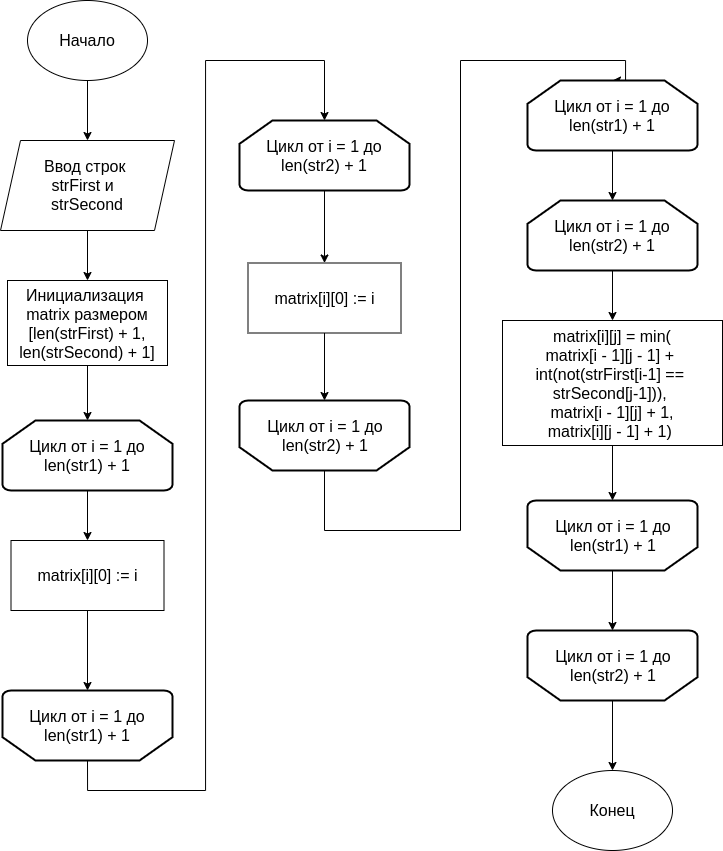
\includegraphics[width=0.6\textwidth]{img/diagramLev.png}
		\caption{Схема алгоритма Левенштейна}}
\end{figure}

\begin{figure}[ht!]
	\centering{
		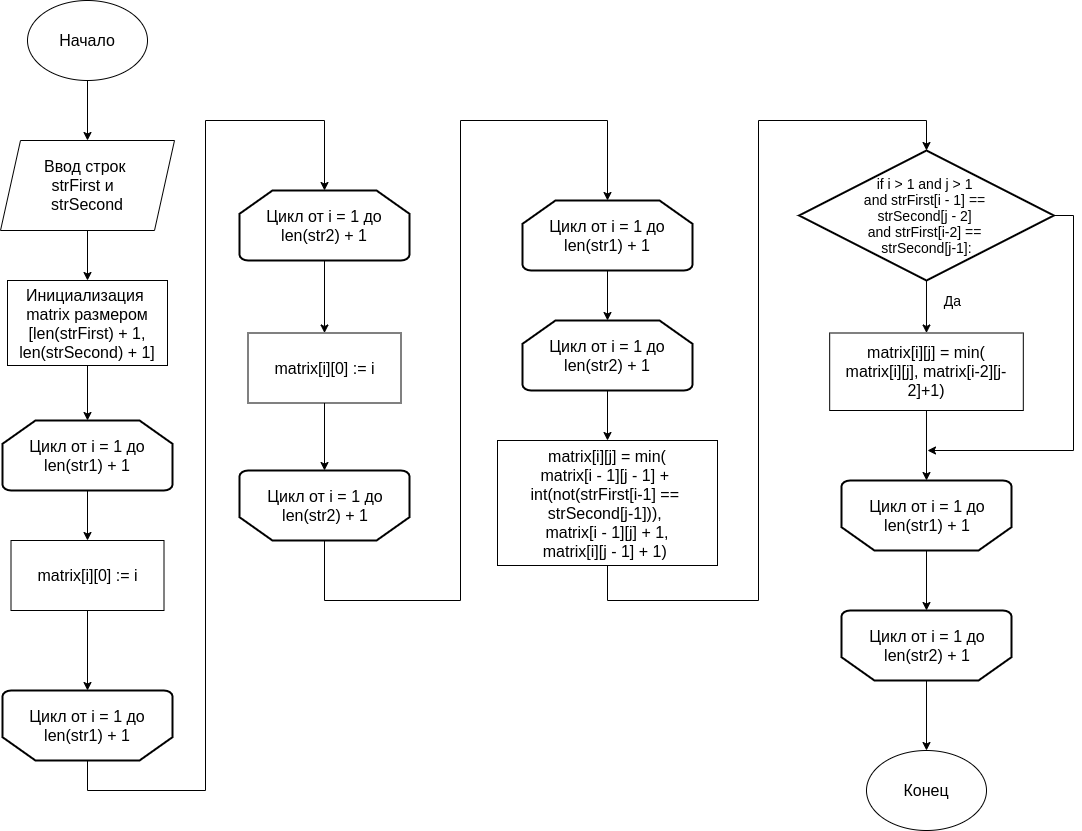
\includegraphics[width=1\textwidth]{img/diagramDamLev.png}
		\caption{Схема алгоритма Дамерау-Левенштейна}}
\end{figure}

\begin{figure}[ht!]
	\centering{
		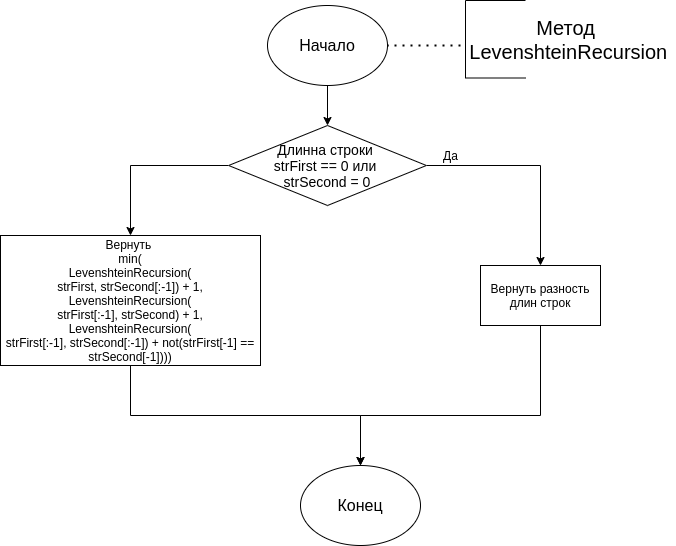
\includegraphics[width=0.8\textwidth]{img/diagramLevRec.png}
		\caption{Схема рекурсивного алгоритма Левенштейна}}
\end{figure}

!!! На рисунке таком-то мы разобрали то-то и то-то
%\section{Вывод}
%
%В данном разделе мы рассмотрели схемы алгоритмов Левенштейна и Дамерау-Левенштейна.